\documentclass{pshscarc}\usepackage{graphicx, color}
%% maxwidth is the original width if it is less than linewidth
%% otherwise use linewidth (to make sure the graphics do not exceed the margin)
\makeatletter
\def\maxwidth{ %
  \ifdim\Gin@nat@width>\linewidth
    \linewidth
  \else
    \Gin@nat@width
  \fi
}
\makeatother

\usepackage{Sweavel}


\usepackage{indentfirst}
%\usepackage{titlesec}
%\titleformat{\section*}[runin]{\Large\bfseries}{\thesection}{\topskip}{\vspace{\topskip}}[\vspace{0pt}]

%% Based on physlb01 class 
%% Last modified 2012.08.28
%%
%% main.tex
%% Based on formatted NIP thesis by Johnrob Y. Bantang (2006)
%%
%% Last modified 2012.03.19 cmnpinol
%%
%% This tex is free; you can redistribute it and/or modify it under
%% the terms of the GNU General Public License as published by the
%% Free Software Foundation version 2. See gpl.txt.
%%
%% This tex files are distributed in the hope that it will be useful,
%% but WITHOUT ANY WARRANTY; without even the implied warranty of
%% MERCHANTABILITY or FITNESS FOR A PARTICULAR PURPOSE.  See the GNU
%% General Public License for more details.
%%
%% You should have received a copy of the GNU General Public License
%% along with this program; if not, write to the Free Software
%% Foundation, Inc., 51 Franklin Street, Fifth Floor, Boston, MA
%% 02110-1301, USA.
%%
%%
%%


   %% square-bracketed, numbered, sorted, and compressed citations
   %% for more info: http://merkel.zoneo.net/Latex/natbib.php
%\usepackage{verbatim} %% for \verbatiminput
%\usepackage{graphicx} %% for the graphics environment%
%\usepackage[centertags]{amsmath}

\usepackage{mathpazo}
\usepackage{microtype}
\usepackage[utf8]{inputenc}
\usepackage[T1]{fontenc}
\usepackage{siunitx}
\usepackage{minted}

\usepackage{pgfplots}
\usepackage{pgfplotstable}
\pgfplotsset{compat=1.7}
\usepackage{array}
\usepackage{booktabs}
\usepackage{threeparttable}

\usepackage{tikz}
\usetikzlibrary{shapes.geometric,positioning,arrows,fit}

\usepackage{placeins}
\usepackage{titlesec}
\titleformat{\section}{\large\bfseries}{\thesection}{0em}{}

\titlespacing{\chapter}{-\baselineskip}{-\baselineskip}{-\baselineskip}

\usepackage[style=biblatex-cse,backend=biber]{biblatex}
\DefineBibliographyStrings{english}{%
  references = {Cited References}}
\addbibresource{yodong.bib}

%% Header section
\title{\textbf{Time Series Analysis of Precipitation in Baguio City between 2001 and 2012 Using Holt-Winters Forecasting}}
\email{author@mail.com}%% apperas only when dfrat version use \draft option.
\adviser{JOSEPH S. TABADERO, JR.}{~}%% Required
\coadviser{MELANIE MATIAS}{~}%
\reader{Conrado C. Rotor, Jr.}{Ph.D.}%% required 
\head{Joseph S. Tabadero, Jr.}{~} %% head
\director{Arfe G. Castillo}{~} %% director
\dean{Conrado C. Rotor, Jr.}{Ph.D.} %% director
\gradyear{2013}\gradmonth{March} %% graduation month and year
\defenseDate{4 March 2013}

%% Specify author details (for abstract, title page and certification page)
\surnamea{Cabantac}
\firstnamea{Sheanne Eric}
\midinitiala{P}
\surnameb{Osbucan}
\firstnameb{Mikhail Antoni}
\midinitialb{A}
\surnamec{Yodong}
\firstnamec{John Christopher}
\midinitialc{C}
%\firstnamed{Analoraine}
%\midinitiald{M}
%\surnamed{Dalilis}
%\surnamee{Author}
%\firstnamee{Fifth}
%\midinitiale{N}
%\surnamef{Author}
%\firstnamef{Sixth}
%\midinitialf{N}

%% 

%% Preliminary pages' contents input here..
\dedication{ \thispagestyle{empty}

\vfill
\begin{center}
\singlespacing
This Research Paper is for our teachers who havenever ceased to teach and guide us, 
to our families who helped us in everything, and to our friends who inspired us  to 
finish this study. Above all, to the Almighty God who provides us wisdom, knowledge 
and perseverance as we have completed this research.
\end{center}
\vfill
\clearpage
\newpage }%% optional, see dedication.tex for sample content.
\biosketch{ \chapter{Biographical Sketch}
\noindent
{\singlespacing
\begin{minipage}{0.3\textwidth}
\includegraphics[width=0.8\linewidth]{Figures/2013-03-04-17-00-28}
\end{minipage}\hfill
\begin{minipage}{0.68\textwidth}
\textbf{John Christopher C. Yodong}, born on October 06, 1996, is a graduate of SPED Center Elementary School and is currently a fourth year student in PSHS-CAR campus. He is a citizen of the Republic of the Philippines and he is a resident of Baguio City. He is a consistent learner and he is able to perform well in school.  He, along with Sheanne Eric P. Cabantac and Mikhail Antoni A. Osbucan, is one of the proponents of the research on the series analysis of rainfall in Baguio City. 
\end{minipage}

\vfill

\noindent
\begin{minipage}{0.68\textwidth}
\textbf{Mikhail Antoni Azul Osbucan} is currently studying at Philippine Science High School. He is currently a member of  the section IV-Photon. He was born on the 30th day of March on 1997 in Baguio City. He is the first child of Ma. Lourdes Osbucan and Rommel Paolo Osbucan. He is of Igorot, Bisayan, and Tagalog decent. He likes to play basketball a lot and he also watches NBA a lot. He is a big fan of alternative music. He is also a big fan of action and suspense movies. When he grows older, he wants to become either a successful pilot or a successful cardiologist. He also believes in the saying that “Hardwork beats talent when talent fails to work hard.” 
\end{minipage}\hfill
\begin{minipage}{0.3\textwidth}\raggedleft
\includegraphics[width=0.8\textwidth]{Figures/IMG_5287}
\end{minipage}

\vfill

\noindent
\begin{minipage}{0.3\textwidth}
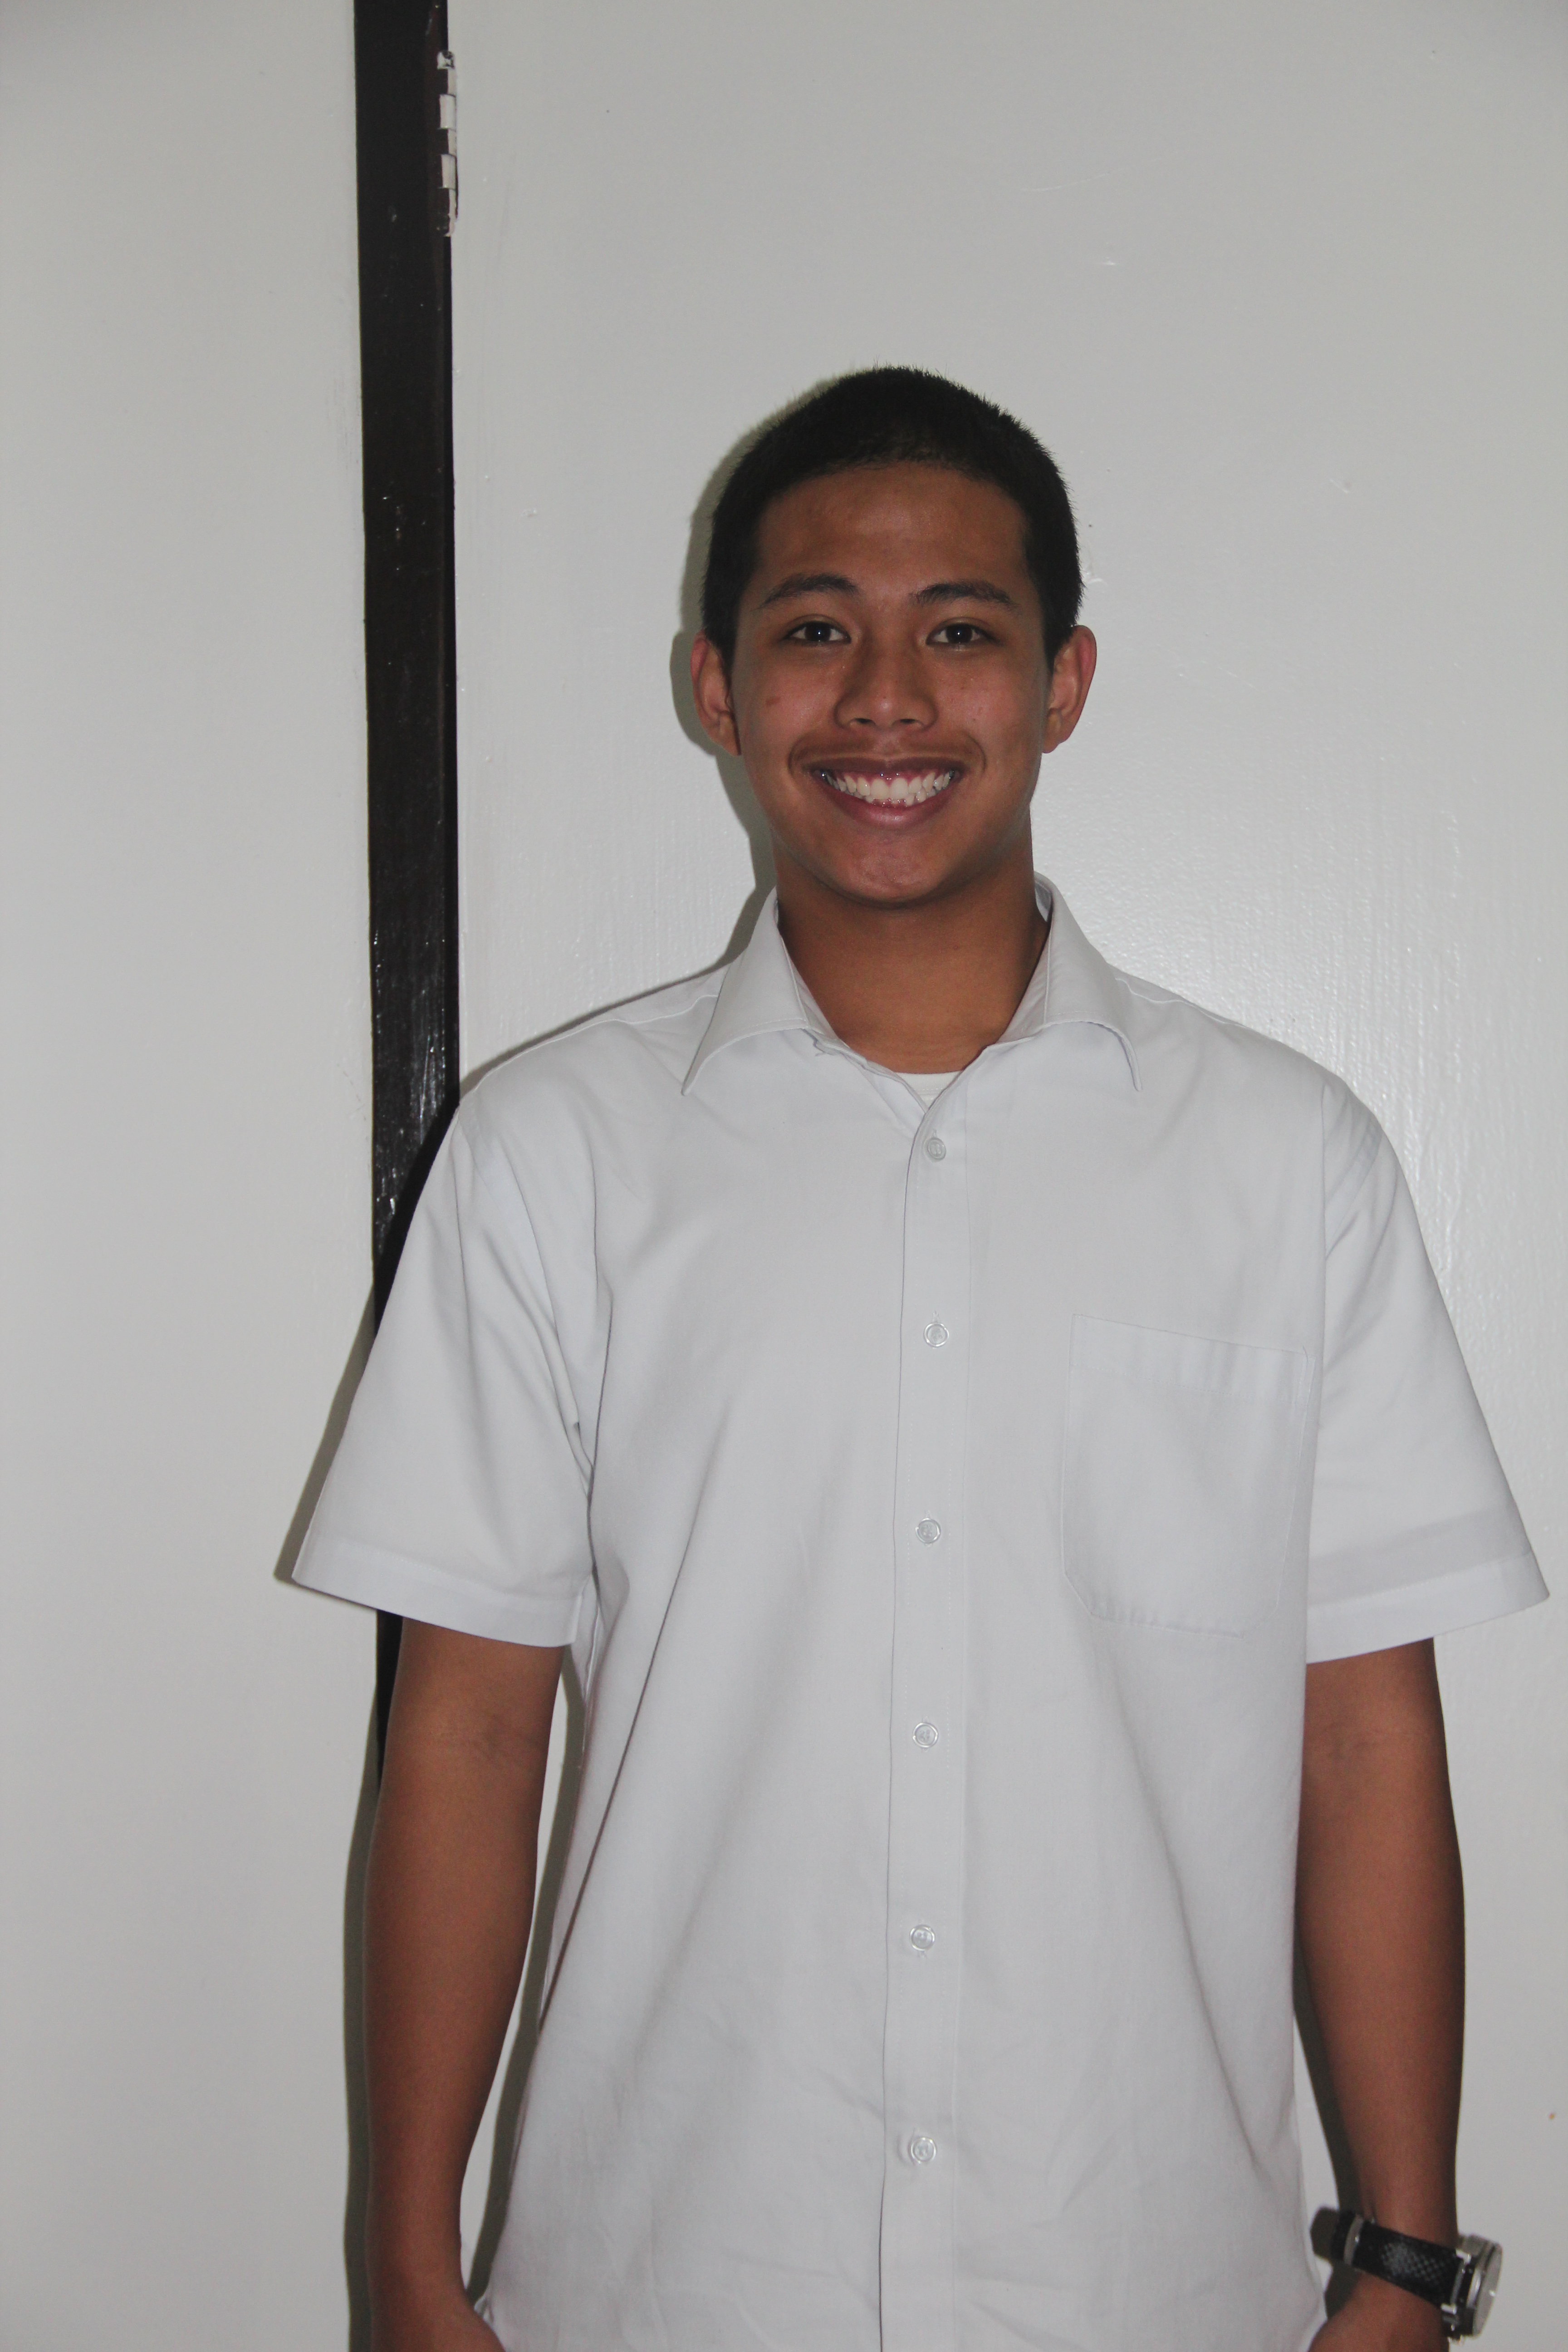
\includegraphics[width=0.8\textwidth, keepaspectratio]{Figures/IMG_5656}
\end{minipage}\hfill
\begin{minipage}{0.68\textwidth}
\textbf{Sheanne Eric P. Cabantac} is a Filipino citizen, born and raised in Baguio City on January 14,1997. He completed his primary education in Star Educational School in La Trinidad and graduated as an academic achiever. He then pursued his elementary education at SPED Center Baguio City, before getting to Philippine Science High School CAR Campus. He is a son to Eduardo R. Cabantac and Sheryl Anne P. Cabantac, and an older brother to three siblings.
\end{minipage}} }%% optional, see biosketch.tex for sample content.
\acknowledgments{ We would like to acknowledge the contributions of the following group and individuals to the development of this thesis paper: 
Our class peer research group for the cooperation and camaraderie. We would also like to thank the Baguio City PAGASA Weather Station and Dr. Salvador Olinares of PAGASA. We are also heartily thankful to our research adviser Mr. Joseph S. Tabadero Jr and our critic reader Ms. Melanie Matias, whose encouragement, guidance and support from the initial to the final level enabled us to develop an understanding of the subject. 
Lastly, we offer our regards and blessings to all of those who supported us in any respect during the completion of the project. 
\begin{flushright}
Cabantac, Sheanne Eric P.\\
Osbucan, Mikhail Antoni A.\\
Yodong, John Christopher C.
\end{flushright}
 } %% optional, see acknowledgment.tex for sample content.
\abstract{ \chapter{ABSTRACT}
{\singlespacing\noindent
\textbf{CABAOIG, RONALD R.}, \textbf{UNICO, BRYAN LORENZO B.}, and \textbf{LAMSIS, NEILBURT GENE M.}, 
Philippine Science High School - Cordillera Administrative Region Campus, March 2013. \textbf{EFFECTS 
OF  BLACK LIGHT ON PECHAY (\textit{Brassica rapa} L. cv group \textit{Pak Choi}}.

\begin{flushleft}
Adviser: \textbf{ARFE G. CASTILLO}\\
Critic Reader: \textbf{CONRADO C. ROTOR, JR., Ph.D.}
\end{flushleft}

The research was created to establish a better understanding on the effects  of black light on 
plants, specifically, the Chinese cabbage, commonly known as pechay. The data weere gathered 
by planting pechay plants and dividing them in equal numbers into three groups.
}

\newpage } %% see abstract.tex


\usepackage{amsmath}
\usepackage{mathpazo}
\usepackage{listings}
\usepackage{inconsolata}
\usepackage{caption}
\captionsetup{skip=5pt,labelfont=bf}
\lstset{breaklines=true,showstringspaces=false,
escapeinside={/*}{*/}
}
\newcommand{\Rstat}{\textsf{R}}


\begin{document}
\maketitle %% creates title page, do not remove this line.
\makePrelim %% creates preliminary pages, do not remove this line.
\listoflistings

\chapter{Introduction}

%\begin{figure}[ht]
%  \centering %%used to center the figure
  %% The width option is used to rescale the figure into the proper
  %% fraction of the \columnwidth
%  \includegraphics[width=0.53\columnwidth]{figures/small.jpg}\\
%  \caption[This appears on List of Figures]
%{This is the caption that appears at the bottom of the figure}
%  \label{small}
%\end{figure}

%\pagebreak % This command forces succeeding text to appear on the next page

%\ref{silofailure}.

%\newpage % same behavior as \pagebreak

	Precipitation is any form of humidity that falls from the clouds in the air to the exterior of the Earth. Since precipitation refers to the liquid quantity and how much of it is isolated on the Earth within a given time, it is measured in volumes and concentration of precipitation on specific areas where the study is focused on. (Ramsey, 1998)
	
	Rain is a group of droplets that tends to fall towards the land of the Earth. The cloud cannot already include the amount of cloud droplets present within it that is why the cloud needs to release these droplets and when they are released, these droplets are already called as rain. Rain is the only type of liquid precipitation, as opposed to non-liquid types of precipitation, which are sleet, snow, and hail. A presence of a thick layer of our atmosphere is needed by rain to maintain temperatures above the melting point of water on the surface of the Earth. When ice crystals within a specific cloud collide against each other, precipitation is formed. Ice crystals have different shapes. There are oblate crystals, round-shaped crystals, and crystals that look like a small sphere. 
(Ramsey, 1998) The major cause of rain production is moisture contrasts that are commonly called as weather fronts and some moisture moving along the zones of temperature. Based on the location of the Philippines, this country only experiences rain, drizzle, and hail among the other types of precipitation. (“Earth Science: The Philippines in Focus,” 1983)

	Since the precipitation is measured in volumes of water in a specific area, the best way to measure the amount of precipitation is to gather all fallen liquid on a specific area with the use of waterproof walls and bases to see how high the water would increase from ground level.  An instrument used in this process with a similar mechanism is the rain gauge.  The rain gauge is the most widely used weather instrument in measuring precipitation.  The rain gauge is composed of a funnel and a cylindrical container where the water accumulates and is collected. However, a rain gauge is most effective when used in a perfectly flat area with its surroundings of the same level.  When used in mountainous regions or areas with uneven ground levels, either the measurements would be inaccurate or multiple rain gauges must be used for each ground level. Rainfall varies in amounts depending on the altitude.  The measurements on a rain gauge are only applicable on a fairly small radius or area around it, any data that would need more information about the amount of rainfall on a specific radius would be erroneous.
	
	The most common rain detector used in electronic weather stations is the “tipping bucket” type of rain sensor.  This fascinating type of technology uses two small “buckets” mounted on a swivel. The tiny buckets are manufactured with tight tolerances to guarantee that they hold an exact quantity of precipitation.  The tipping bucket assembly is to be found underneath the rain collector, which funnels the precipitation to the buckets.  As rainfall fills the tiny bucket, it becomes overbalanced and tips down, emptying itself as the other bucket pivots into place for the next reading. The action of each tipping episode triggers a small control that activates the electronic circuitry to transmit the count to the indoor console.  On a wireless rain gauge, records are transmitted through a radio signal. (“WW2010,” 2003)
	
	These methods aforementioned are some methods that PAGASA Weather Station is implementing to gather records of rainfall during the entire day, where they collect data every after three hours starting at two in the morning until eleven in the evening.
	
	The PAGASA Weather Station, also recognized as Philippine Atmospheric, Geophysical and Astronomical Services Administration, is a nationwide institution of the Philippines that provides warnings about flood and typhoon.  They also provide a lot more services like public advisories and forecasts concerning the up to date weather report of the country.  PAGASA furthermore provides meteorological, astronomical, and climatological information for the security of life and property of the Filipino people.  This government agency started operating on the 8th of December in 1972.
	
	This agency has a mandate that states that they need to provide protection against natural calamities to ensure the safety of the Filipino citizens, well-being and economic security of all the people, and for promotion of national progress.
	
	Residents in the Philippines would expect to have a huge amount of rainfall every month of the year.  The rainy season starts on the end of May and ends on late November or early December. (“Earth Science: The Philippines in Focus,” 1983)
	
	In Batanes, Northeastern Luzon, Western part of Camarines Norte, Camarines Sur, Albay, Bondoc Peninsula, Eastern Mindoro, Marinduque, Western Leyte, Northeastern Cebu, Bohol, and most of the Central and Southern Mindanao experience rainfall that us more or leass evenly distributed all throughout the year. (“Earth Science: The Philippines in Focus,” 1983)
	
	Upon observing the rainfall pattern in Baguio City, the proponents also observed some factors that could massively affect the rainfall in our city.  One factor that would affect the rainfall pattern of Baguio City is the season.  According to some references, high precipitation occurs during the humid season of the year while low precipitation occurs during the dry season of the year. Since the city is located at a high altitude, the elevation could also affect the pattern of rainfall that will occur.  Mountains affect the amount of rainfall.  Rains fall more often on the slopes facing the wind than on the slope away from the wind. The reason is that a wind hitting the side of the mountain tends to rise along the slope reaching heights of low temperature.  There, the moisture in the wind condenses to form rain.  By the time it reaches the other side of the mountain there is not enough amount of moisture to further condense.  The eastern coastal areas generally receive more rainfall than the western parts.  The eastern areas have high rainfall from October to March when the monsoon blows over the country.  For the Philippines as a whole, June to December are the rainy months while January to May are the dry months. (“Earth Science: The Philippines in Focus,” 1983)

\addcontentsline{toc}{section}{Background of the Study}
\section*{Background of the Study}

Baguio City is a highly urbanized city located in the province of Benguet.  It has an altitude of 1610 meters and covers a total land are of 57.5 \si{\square\kilo\meter}. Landslide and flashflood occurrences are highly unpredictable in some areas of the city because rainfall amount does not have a recognizable pattern.  Thus, many parts of Baguio City are suffering from landslides and flashfloods during periods of unpredicted heavy rainfall.  In order to increase the safety, awareness against such environmental disasters and an analysis regarding the rainfall patterns of Baguio City has to be done to provide basic information.

	Such study has been done in different countries such as Northeastern Thailand, India, and Australia.  The necessary data shall be collected from the weather station of Baguio City to produce a forecast for the amounts of rainfall every year.
	
\addcontentsline{toc}{section}{Statement of the Problem}
\section*{Statement of the Problem}

	The amount of precipitation in Baguio City has become very unpredictable, to a point where landslides and flashfloods have become unforeseeable. The aim of the study is to provide a basic forecast about how much precipitation would fall on Baguio City on the succeeding year, based on the ten-year data gathered from PAGASA.

%
%\addcontentsline{toc}{section}{Scope and Limitation of the Study}
%\section*{Scope and limitation of the study}
%
%\addcontentsline{toc}{section}{Time and place of study}
%\section*{Time and place of study}
\addcontentsline{toc}{section}{Significance of the Study}
\section*{Significance of the study}

This study can be a reference for preparations for certain agricultural activities like cultivating, planting, and harvesting.  It can also be a reference as a precautionary measure for flash floods and landslides.

\addcontentsline{toc}{section}{Scope and Delimitation}
\section*{Scope and Delimitation}

The study is limited only to analyzing rainfall amounts and no other weather factors.  The study has been limited to only analyzing the rainfall amounts in Baguio City because it ensures the safety of the researchers and it gives the easiest access to the needed data. This study was also limited to determining the coefficients of the Holt-Winters additive seasonal model and not all the set of the equations in the model. This study is further delimited to the prediction of the average monthly rainfall for the months of 2012.

\addcontentsline{toc}{section}{Definition of Terms}
\section*{Definition of Terms}

For clearer understanding of terms used in this study, below are the operational definitions of the terms used in this research paper.

\textbf{Time series analysis} concerns the analysis of data collected over time. Usually
the intent is to discern whether there is some pattern in the values collected
to date, with the intention of \textit{short term} forecasting

\textbf{Seasonality} is defined to be the tendency
of time-series data to exhibit behavior that repeats itself over regular periods.

\textbf{Additive seasonality} shows steady seasonal fluctuations, regardless of the overall level of the series.

\textbf{Multiplicative seasonality}, the size of the seasonal fluctuations vary,
depending on the overall level of the series.

\textbf{Exponential smoothing} is a procedure for continually revising a forecast in the light of more recent experience. Exponential Smoothing assigns exponentially decreasing weights as the observation get older. In other words, recent observations are given relatively more weight in forecasting than the
older observations.

\textbf{Forecasting} is the process of making projections about future performance on the basis of historical and current data.

\textbf{Holt-Winters} is a set of equations which handle time series data that show trend, seasonality, and a random effects.

\textbf{Additive Seasonal Model} is the Holt-Winters model used when the data exhibits Additive seasonality. In this model, we assume that the time series is represented by the model

\begin{equation}
y_t = a + b t + S_t + \epsilon_t
\end{equation}
where,
\begin{flushleft}
$y_t$ response of interest at time $t$\\
$a$ is the base signal also called the permanent component\\
$b$ is a linear trend component\\
$S_t$ is a additive seasonal factor\\
$\epsilon_t$ is the random error component\\
Let the length of the season be $L$ periods.\\
\end{flushleft}
The seasonal factors are defined so that they sum to the length of the season, that is

\begin{equation}
\sum_{1\le t\le L} S_t = 0.
\end{equation}
The trend component $b$ if deemed unnecessary, maybe deleted from the model.

The application of the model and further description of the rest of the set of equations in the model can be found in Kalekar (2004, p 7).

\textbf{Precipitation} is a deposit on earth of hail, mist, rain, sleet, or snow. It is also the quantity of water deposited.

\textbf{Rainfall} is the amount of precipitation usually measured by the depth in millimeters.

\textbf{Rainy day} refers to the period where precipitation occurs at any time of the day.
\chapter{Review of Related Literature}

\section*{Time Series Analysis on hourly rainfall (Cutrim et al 2000)}

Time Series Analysis was used on an average hourly precipitation. The method determined whether statistically significant differences existed from each season. The data gathered is a 20-year period consisting of 2-hour intervals per day. In a seasonal analysis it was defined that winter, spring, summer, and fall are the seasons to be used. The Box-Jenkins methodology, a sample autocorrelation function (ACF) and a partial auto correlation function (PACF) plot were employed for each of the 12 periods of the day, for both precipitation accumulations and counts. A plot of ACF values at different lags was used to find a working series of stationary time points for the precipitation parameters accumulation and counts. For both precipitation parameters, the ACF plots clearly indicated the time series to be a non-seasonal component, but the same plot showed the need for further differencing of the seasonal component of the series, which occurs every four time periods. The periods of differencing, therefore, are 1 for the seasonal component of order 4. This differencing scheme produced a stationary time series, which is a prerequisite in ARIMA Modeling. 

The ACF and PACF plots of the differentiated series were then used to determine the autoregressive (AR) component and a moving average (MA) component of the series. Except for precipitation count at 6 a.m. the ARIMA model for cache of the differenced precipitation time series year were identified. (See Figure \eqref{newpic}).

\begin{figure}[!ht]
\centering
\includegraphics[width=4in, keepaspectratio]{daily}
\caption{\label{newpic} Time Series Analysis on a 50 year data of rainfall and temperature (Cutrim et al 2000).}
\end{figure}

A large set of data involving more than 50 years of rainfall and temperature data were examined using Spectral Analysis, Time Series Analysis-ARIMA Methodology to analyse climatic trends and interactions. Fourier analysis, linear regression and ARIMA based time series models were used to analyze the large data sets using Mat-lab, SPSS and SAS programs. The results that came up showed that the rainfall data was variable and appeared seasonal while the temperature data appeared stationary. Spectral analysis also showed variations in rainfall and temperature over 50-60 years but the results showed that rainfall and temperature varied coherently, with a cycle of about 2-3 years. An inverse relationship in trend was noted between rainfall and daily temperature range using linear regression among the variables. The ARIMA models showed autocorrelation and seasonality providing time series models.

It was concluded that: There is a cyclic pattern noted in both the rainfall and temperature time series and a cycle of about 3 years in the rainfall and temperature data sets suggesting a coherent variance in the relationship. This finding suggested a cyclic nature of large rainfall events over time and was confirmed by the recent large rainfalls events in 2009-10. Linear regression showed an inverse relationship in trend between rainfall and temperature range only even though the r value was around 0.27. 

\section*{Time Series Analysis on the Agricultural\\ Commodities Prices}

Other than prices, the data includes variables reflecting demand and supply factors affecting agricultural prices. Series are on a monthly basis. On the demand side it has been considered that monetary aggregate will be the proxy for world real aggregate expenditure, production of ethanol and biodiesel, several proxies for trading activity in futures markets, and the U.S. dollar–Euro exchange rate. On the supply side the price of oil, price of fertilizers, and volume of exports by major world producers are used. 

The data gathered was from 2002 to 2009. The end of the series was restricted due to unavailable data, and restrictions at the beginning of the series were due to the presence of structural changes based on Chow tests. All price data and other variables will be taken in log form when analyzed.

\section*{The distribution of monthly rainfall}

Monthly distributions of rainfall in space and time can provide guidelines for crop scheduling and for introducing better cropping patterns in the region.

To determine the periodicity of the monthly rainfall sequence at a station, the method developed by Vujica M. Yevjevich was used, in which the parameters involved are clearly defined. 

It was found that monthly rainfall sequences at all the stations under consideration
have six significant harmonics, which means that the monthly rainfall has a periodic part that consists of components corresponding to the following six periods: 12, 6, 4, 3, 2.4 and 2 months. The variances of the monthly means and the monthly standard deviations are explained up to more than 90\%  by these six significant harmonics. These findings show that after removing the first six periodic components, the residual rainfall sequence at a station can be considered to be stationary at least in the mean and standard deviation. (See Table 1.)

For most cases, the serial correlation coefficient between two successive monthly
rainfall sequences at a station were found not to be significantly different from zero. Nonsignificance of correlation does not necessarily imply statistical independence, monthly rainfall totals were analysed separately and a probability distribution was fitted month by month.

\begin{table}
\centering
\begin{tabular}{ccc}
\toprule
Station & Mean & Standard Deviation\\
\midrule
Buriram & 0.925 & 0.917\\
Chaiyaphum & 0.940 & 0.938\\
Kalasin & 0.924 & 0.920\\
Khon Kaen & 0.927 & 0.937\\
Loei & 0.924 & 0.921\\
Maha Sarakham & 0.935 & 0.921\\
Nakhon Phanom & 0.924 & 0.979\\
Nakhon Ratchasima & 0.931 & 0.920\\
Nongkhai & 0.919 & 0.929\\
Roi Et & 0.922 & 0.919\\
Sakhon Nakhon & 0.917 & 0.941\\
Ubon Ratchatani & 0.922 & 0.942\\
Udon Thani & 0.917 & 0.927\\
Yasothon & 0.927 & 0.939\\
\bottomrule
\end{tabular}
\caption{\label{tab:first} The residual rainfall sequence in agricultural provinces in Thailand.}
\end{table}

It was concluded that each monthly rainfall sequence has a periodic part consisting of six constituents corresponding to the following six periods: 12, 6. 4, 3, 2.4 and 2 months.
At each station the rainfall sequence in a month is independent of the rainfall sequences in the other months. Since many monthly rainfall sequences in the Northeast have zero values, the leakage law is most appropriate for fitting these sequences. Monthly rainfall in the region varies greatly from month to month, resulting in high degrees of irregularity, ranging from 45 to 70 per cent. Monthly rainfall also varies greatly from year to year as indicated by the high values for the coefficient of variation. The eastern and north-eastern sections of the region are the wettest areas of the Northeast from April to September but they are the driest parts from October to December. The maximum amount of rainfall for the entire region usually occurs in August or September while the minimum normally occurs in December or January.
\chapter{Methodology}

%\section{Materials}

% Below is an environment for itemized lists.
%\hspace{\parindent}The materials used in this study are the following:
%\begin{itemize}
%  \item Uncooked tapioca “sago” balls 
%  \item Digital weighing scale (Max. capacity: 200g, Resolution: 0.001g)
%  \item Cylinder tube made of cardboard: opaque and open in both ends
%  \item Plywood
%  \item 100mL graduated cylinder
%  \item Plastic/cellophane bags
%  \item Plastic cups
%\end{itemize}

%\clearpage
\addcontentsline{toc}{section}{Research Design}
\section*{Research Design}

The study, which is about the rainfall patterns of Baguio, involves quantitative research on the rainfall amounts of Baguio. A statistical analysis shall be done on the gathered data, particularly a Time Series Analysis. The Holt-Winters Method will be applied to the time series data from January 2001 to December 2011 to make determine the coefficients of the mathematical model for forecasting values from January 2012 to December 2012 which were retrieved from PAG-ASA. Auto-correlation function, Ljung-Box test, and test for normality were used to test for the validity of the model.

\addcontentsline{toc}{section}{Sources of Data}
\section*{Sources of Data}

The data were the rainfall amounts per month in Baguio City. The sample, which will be taken from the population, were the rainfall amounts ranging from January 2000 to December 2011. Rainfall amount was measured using either a tipping bucket or rain gauge. It is measured and recorded in millimeters every three hours starting from 2a.m. to 11p.m.. The data was gathered from the weather station of PAGASA located in Baguio City.

\addcontentsline{toc}{section}{Locale of the Study}
\section*{Locale of the Study}

There have been a series of occurrences of unforeseen flashfloods and landslides in Baguio City, especially in areas such as City Camp Lagoon, so the researchers chose that the study should be done in Baguio City.

\addcontentsline{toc}{section}{Population/Sampling}
\section*{Population/Sampling}

The study involved the analysis of rainfall amounts gathered daily by PAGASA. The research would only take into consideration the data gathered from January 2000 to December 2011 since the study was proposed before several months before the year 2012 ended.

\addcontentsline{toc}{section}{Instrumentation and Data Collection}
\section*{Instrumentation and Data Collection}

The data was then summarized and classified by year on Microsoft Excel. However, the amount of rainfall for May 2006 was missing, so a statistical method called Bootstrapping method was done to generate a forecasted value. 

Bootstrapping method is a method developed by B. Efron on 1979. It is a computer-based method for assigning accurate sample estimates. This method allows estimation of the sample distribution of almost any value using only very simple methods (Varian 2005). Using R-statistics, a computer statistical software, bootstrapping method was used to generate an estimate for May 2006. 

The data from January 2001 to December 2005 was used to generate an estimate for May 2006, through R-statistics.
Then, a time-series analysis was conducted. A time-series analysis is a method used to obtain an understanding of the forces, which produced the data. The time series analysis is a set of data used and collected sequentially at fixed intervals of time. The amount of rainfall , is a time series data, which is measured and recorded at successive time intervals.

\FloatBarrier
\addcontentsline{toc}{section}{Protocol}
\section*{Protocol}

The time series analysis and forecasting will be done using a statistical software called R-statistics. R is a free software environment for statistical computing and graphics. It compiles and runs on a wide variety of UNIX platforms, Windows and MacOS. 

\newpage
\addcontentsline{toc}{section}{Research Paradigm}
\section*{Research Paradigm}
\tikzset{
input/.style={draw,trapezium, trapezium left angle=70, trapezium right angle=110, align=center},
process/.style={draw,rectangle,align=center},
decision/.style={draw, diamond, align=center},
}
\begin{figure}[!ht]
\centering
\begin{tikzpicture}[ultra thick,rounded corners, >=stealth']
\node (Data) [input] {Data};
\node (Pre-process) [process, below=of Data] {Pre-processing\\ stage:\\
	Encoding\\
	and\\
	Inputting to\\
	Software
	};
\node (holt) [process, below=of Pre-process] {Holt-Winters\\
exponential\\
smoothing\\
and\\
forecasting};
\node (box) [process, below=2.5cm of holt] {Ljung-Box test};
\node (acf) [process, left=of box] {
Auto-correlation\\
function\\
technique
};
\node (normal) [process, right=of box, inner sep=12pt] {
Test \\
for normality
};
\node (stat) [fit=(normal)(box)(acf), process, inner sep=24pt] {
};
\node (model) [below=2.5cm of box, process]{
Model
};

\foreach \x/\y in 
	{Data/Pre-process,Pre-process/holt,holt/stat,stat/model}
	\path [->] (\x) edge (\y);

\node at (stat.north) [anchor=north] {
\textbf{Tests for Fitness of Holt-Winters Model}
};
\end{tikzpicture}
\caption{\label{flowchart} Flow chart for time rainfall time series analysis.}
\end{figure}

 %%could be model or experiment set-up
\chapter{Results and discussion}

Table \eqref{tab:rawdata} shows the raw data from January of 2001 to December of 2012. The initial data collected were from January 2001 to December 2011. The rainfall data for January 2012 to December 2012 were collected after one year for comparison of the predicted values. The data for May 2006 was initially missing. Using bootstrapping method in \texttt{R}, the missing May 2006 data was generated.

\begin{table}[!ht]
\caption{Amount of Precipitation Per Month in mm, from 2001 to 2012}
\begin{threeparttable}
\resizebox{\linewidth}{!}{
\pgfplotstabletypeset[header=true,
font=\small,
every head row/.style={
before row=\toprule,
after row=\midrule,
},
every last row/.style={
after row=\bottomrule},
string type
]{rawdata.dat}
}
\begin{tablenotes}
\item [$\star$] Trace amount, $< 0.01$ mm
\item [$\triangle$] Bootstrapped value
\end{tablenotes}
\end{threeparttable}
\label{tab:rawdata}
\end{table}

\section*{Analysis of Data}

The data was saved in a file named \texttt{baguiorainfall.dat}. This data was then inputted in \Rstat{} and stored in a variable \texttt{baguiorainseries} using the \texttt{ts} function.

\begin{Schunk}
\begin{Sinput}
baguiorain <- read.table("baguiorainfall.dat")
baguiorainseries <- ts(baguiorain, frequency = 12, start = c(2001, 1))
\end{Sinput}
\end{Schunk}


Figure \eqref{fig:TSPlot} shows the graph of the rain fall time series from January 2001 to December 2011. It can be seen that the data is seasonal, peaking every July to August every year.

\begin{figure}[!ht]
\centering
\begin{Schunk}
\begin{Sinput}
plot.ts(baguiorainseries)
\end{Sinput}

\includegraphics[width=.7\textwidth]{figure/listings-YeastBoxPlot} \end{Schunk}


\caption{\label{fig:TSPlot} Plot of Baguio rain fall time series, from January 2001 to December 2011.}
\end{figure}

Here, the time series data is broken down into its components. This is done in preparation to eliminating the seasonal component of the data. Only the partial results are shown in \eqref{fig:Components}. The full results are in Listing \eqref{fig:Components2}.

\begin{center}
\captionof{figure}{\label{fig:Components} Partial results of the seasonal, trend, and random components.}
\begin{Schunk}
\begin{Sinput}
baguiorainseriescomponents <- decompose(baguiorainseries)
baguiorainseriescomponents
\end{Sinput}
\begin{Soutput}
$x
          Jan      Feb      Mar      Apr      May      Jun      Jul
2001   14.600   39.500  289.800   76.000  291.000  451.400 1642.000
2002    5.000    2.000    0.600   71.200  264.400  411.000 1883.400
2003    9.800   25.400    4.800   46.800  662.700  792.400  721.300
.
.
.

          Aug      Sep      Oct      Nov      Dec
2001  274.000  842.200   97.000   61.600   23.200
2002  525.600  301.500  224.800   67.300   10.000
2003 1089.400  303.200  179.700   60.400    4.400
.
.
.

$seasonal
         Jan     Feb     Mar     Apr     May     Jun     Jul     Aug
2001 -296.55 -293.19 -283.56 -235.99   80.13  204.37  561.21  522.65
2002 -296.55 -293.19 -283.56 -235.99   80.13  204.37  561.21  522.65
2003 -296.55 -293.19 -283.56 -235.99   80.13  204.37  561.21  522.65
.
.
.
         Sep     Oct     Nov     Dec
2001  122.05  128.05 -212.33 -296.84
2002  122.05  128.05 -212.33 -296.84
2003  122.05  128.05 -212.33 -296.84
.
.
.

$trend
       Jan   Feb   Mar   Apr   May   Jun   Jul   Aug   Sep   Oct   Nov
2001    NA    NA    NA    NA    NA    NA 341.5 339.5 325.9 313.6 312.3
2002 317.9 338.4 326.4 309.2 314.8 314.4 314.1 315.3 316.4 315.6 331.2
2003 331.1 306.2 329.8 327.9 325.8 325.3 325.3 329.9 337.4 340.1 330.0
.
.
.

       Dec
2001 309.5
2002 363.7
2003 341.6
.
.
.

$random
          Jan      Feb      Mar      Apr      May      Jun      Jul
2001       NA       NA       NA       NA       NA       NA  739.334
2002  -16.360  -43.257  -42.248   -2.012 -130.491 -107.820 1008.092
2003  -24.773   12.401  -41.398  -45.158  256.792  262.771 -165.233
.
.
.

          Aug      Sep      Oct      Nov      Dec
2001 -588.150  394.268 -344.686  -38.390   10.510
2002 -312.329 -136.973 -218.836  -51.528  -56.807
2003  236.821 -156.201 -288.458  -57.242  -40.400
.
.
.

$figure
 [1] -296.55 -293.19 -283.56 -235.99   80.13  204.37  561.21  522.65
 [9]  122.05  128.05 -212.33 -296.84

$type
[1] "additive"

attr(,"class")
[1] "decomposed.ts"
\end{Soutput}
\end{Schunk}
\end{center}

It can be seen in Figure \eqref{fig:Components} that the data is of additive type. The plot is in Figure \eqref{fig:ComponentsPlot}. 

\begin{figure}[!ht]
\centering
\begin{Schunk}
\begin{Sinput}
plot(baguiorainseriescomponents)
\end{Sinput}

\includegraphics[width=.7\textwidth]{figure/listings-ComponentsPlot} \end{Schunk}


\caption{\label{fig:ComponentsPlot} The plot of the components of the rainfall time series data.}
\end{figure}

To use exponential smoothing to make forecasts for the time series of monthly rainfall in Baguio City, the \texttt{HoltWinters()} function was used.

\begin{figure}[!ht]
\begin{Sinput}
rainforecasts <- HoltWinters(raintimeseries)
rainforecasts
\end{Sinput}
\begin{Soutput}
Holt-Winters exponential smoothing with trend and additive seasonal component.

Call:
 HoltWinters(x = raintimeseries) 

Smoothing parameters:
 alpha:  0.001826 
 beta :  0.422 
 gamma:  0.3554 

Coefficients:
         [,1]
a    267.1477
b      0.5062
s1  -208.3311
s2  -227.2503
s3  -194.1851
s4  -136.7234
s5   147.8871
s6   216.3476
s7   338.7154
s8   673.8567
s9   321.0458
s10  430.4775
s11 -130.6776
s12 -215.8636
\end{Soutput}
\caption{\label{fig:HoltWSmoothing} The output of \texttt{HoltWinters()} function.}
\end{figure}

The output of \texttt{HoltWinters()} made forecast for the same time period covered by the original time series, the time series included rainfall for Baguio City for the period January 2000 to December 2011. So the forecasts were also for that period. An $\alpha$ of 0.001826 indicates that the forecasts were based on both recent and less recent observations--although somewhat more weight was placed on recent observations (Coghlan 2011). A $\beta$ of $0.422$ and a low $\gamma$ of 0.3554 meant that the estimate
of both the trend and seasonal components at the current time point are based upon both recent
observations and some observations in the more distant past. The graph of the original time series against the fitted forecast of the model can be seen in Figure \eqref{fig:fittedgraph}.
\newpage
\begin{center}
\begin{Schunk}
\begin{Sinput}
plot(baguiorainseriesforecasts)
\end{Sinput}

\includegraphics[width=.7\textwidth]{figure/listings-fittedgraph} \end{Schunk}

\captionof{figure}{\label{fig:fittedgraph} The original rainfall time series with the predicted values of the derived model in the same period.}
\end{center}

The output of \texttt{HoltWinters()} function was stored in the variable\newline \texttt{baguiorainseriesforecasts\$fitted}. The forecast for the period January 2000 to December 2011 is shown partially in Figure \eqref{fig:fitted}, and in full in Figure \eqref{fig:fitted2} of \textbf{Appendix B}.

\begin{figure}[!ht]
\begin{Schunk}
\begin{Sinput}
baguiorainseriesforecasts$fitted
\end{Sinput}
\begin{Soutput}
            xhat   level
Feb 2001   14.60   14.60
Mar 2001   27.22   27.22
Apr 2001  160.31  160.31
May 2001  117.58  117.58
Jun 2001  205.48  205.48
.
.
.
Oct 2011  790.45  790.45
Nov 2011  558.28  558.28
Dec 2011  316.67  316.67
\end{Soutput}
\end{Schunk}

\caption{\label{fig:fitted} The forecast for the period January 2000 to December 2011 using Holt Winters.}
\end{figure}

We now make forecasts for further time points by using the
\texttt{forecast.HoltWinters()} function in the R \texttt{forecast} package. \texttt{forecast.HoltWinters()} uses the predictive model derived using the HoltWinters() function. The result is in Figure \eqref{fig:Forecast2}.

\begin{center}
\begin{Schunk}
\begin{Sinput}
library(forecast)
\end{Sinput}
\begin{Soutput}
This is forecast 4.01 
\end{Soutput}
\begin{Sinput}
baguiorainseriesforecasts2 <- forecast.HoltWinters(baguiorainseriesforecasts, 
    h = 12)
baguiorainseriesforecasts2
\end{Sinput}
\begin{Soutput}
         Point Forecast   Lo 80  Hi 80   Lo 95  Hi 95
Jan 2012          59.32 -366.29  484.9 -591.60  710.2
Feb 2012          40.91 -384.70  466.5 -610.01  691.8
Mar 2012          74.48 -351.14  500.1 -576.44  725.4
Apr 2012         132.45 -293.17  558.1 -518.48  783.4
May 2012         417.57   -8.06  843.2 -233.37 1068.5
Jun 2012         486.53   60.90  912.2 -164.42 1137.5
Jul 2012         609.41  183.77 1035.0  -41.56 1260.4
Aug 2012         945.05  519.40 1370.7  294.07 1596.0
Sep 2012         592.75  167.08 1018.4  -58.25 1243.7
Oct 2012         702.69  277.01 1128.4   51.66 1353.7
Nov 2012         142.04 -283.66  567.7 -509.02  793.1
Dec 2012          57.36 -368.37  483.1 -593.73  708.4
\end{Soutput}
\end{Schunk}
\begin{Sinput}
rainforecasts$SSE
\end{Sinput}
\begin{Soutput}
[1] 13193425
\end{Soutput}


\captionof{figure}{\label{fig:Forecast2} The 12-month forecast for the year 2012 based on \texttt{Holt Winters} smoothing.}
\end{center}

Figure \eqref{fig:predgraph} shows the original time series with the graph of the predicted values (in blue color) and the low and high values (shown in light blue-gray color).

\begin{center}
\centering
\includegraphics[width=0.7\maxwidth,height=3.5in]{figure/listings-HWComputations3}
\captionof{figure}{\label{fig:predgraph} The graph of the time series with the forecasted values.}
\end{center}

The ‘forecast errors’ are calculated as the observed values minus predicted values, for each time point. We can
only calculate the forecast errors for the time period covered by our original time series, which is January 2011 to December 2011 for
the rainfall data. One measure of the accuracy of the predictive model is the sum-of-squared-
errors (SSE) for the in-sample forecast errors.
The in-sample forecast errors are stored in the named element “residuals” of the list variable returned by \texttt{forecast.HoltWinters()}. If the predictive model cannot be improved upon, there should be no correlations between
forecast errors for successive predictions. In other words, if there are correlations between forecast errors for
successive predictions, it is likely that the  exponential smoothing forecasts could be improved upon by
another forecasting technique. The function \texttt{acf()} function was used here to test for autocorrelation in the errors.

\begin{Sinput}
acf(rainforecasts2$residuals, lag.max = 20)
\end{Sinput}

\begin{center}
\includegraphics[width=0.7\maxwidth,height=3.5in]{figure/listings-HWComputations4}
\captionof{figure}{\label{fig:acf} \texttt{acf()} output.}
\end{center}

Here the correlogram shows that the sample autocorrelation for the in-sample forecast errors at lags 1 and 11 exceed
the significance bounds. This is more than the 1 than the one in 20 of the autocorrelations for the first twenty lags to
exceed the 95\% significance bounds by chance alone indicating possible auto-correlation in internal errors. 

\begin{Sinput}
Box.test(rainforecasts2$residuals, lag = 20, type = "Ljung-Box")
\end{Sinput}
\begin{Soutput}

	Box-Ljung test

data:  rainforecasts2$residuals 
X-squared = 23.91, df = 20, p-value = 0.2465
\end{Soutput}
\begin{Sinput}
plot.ts(rainforecasts2$residuals)
\end{Sinput}

The Ljung-Box test, with p-value of 0.2465 on the other hand shows no evidence of non-zero autocorrelations in the in-sample forecast errors at lags 1-20.

To be sure that the predictive model cannot be improved upon, the researchers checked whether the forecast errors are normally distributed with mean zero and constant variance. To check whether the forecast errors have
constant variance, the researchers made a time plot of the in-sample forecast errors:

\begin{center}
\begin{Sinput}
plot.ts(rainforecasts2$residuals)
\end{Sinput}

\includegraphics[width=0.7\maxwidth, height=3.5in]{figure/listings-HWComputations5}
\captionof{figure}{\label{insampleerrors}Plot of the in-sample forecast errors.}
\end{center}

The plot shows that the in-sample forecast errors seem to have roughly constant variance over time with some fluctuations between 2000 and 2011.

To check whether the forecast errors are normally distributed with mean zero, a histogram of the forecast errors, with an overlaid normal curve that has mean zero and the same standard deviation as the distribution
of forecast errors can be plotted. Here the R function \texttt{plotForecastErrors()} was used.

\begin{Sinput}
plotForecastErrors <- function(forecasterrors) {
    # make a red histogram of the forecast errors:
    mybinsize <- IQR(forecasterrors)/4
    mymin <- min(forecasterrors) * 3
    mymax <- max(forecasterrors) * 3
    mybins <- seq(mymin, mymax, mybinsize)
    hist(forecasterrors, col = "red", freq = FALSE, breaks = mybins)
    # freq=FALSE ensures the area under the histogram = 1
    mysd <- sd(forecasterrors)
    # generate normally distributed data with mean 0 and standard deviation
    # mysd
    mynorm <- rnorm(10000, mean = 0, sd = mysd)
    myhist <- hist(mynorm, plot = FALSE, breaks = mybins)
    # plot the normal curve as a blue line on top of the histogram of
    # forecast errors:
    points(myhist$mids, myhist$density, type = "l", col = "blue", lwd = 2)
}
plotForecastErrors(rainforecasts2$residuals)
\end{Sinput}

\begin{center}
\includegraphics[width=0.7\maxwidth,height=3.5in]{figure/listings-HWComputations6}
\captionof{figure}{\label{fig:normalplot} A histogram of the forecast errors, with an overlaid normal curve that has mean zero and the same standard deviation as the distribution of forecast errors.}
\end{center}

The plot shows that the distribution of forecast errors is roughly centred on zero, and is more or less normally
distributed, although it seems to be slightly skewed to the right compared to a normal curve. However, the right
skew is relatively small, and so it is plausible that the forecast errors are normally distributed with mean zero.

%Finally, we use t-test for the predicted values and the actual values for 2012 taken from PAGASA.
%
%\begin{Sinput}
%actual <- c(17.5, 80.3, 151.9, 72.6, 207.7, 659, 1020.2, 2207, 288.3, 72.4, 
%    57.8, 10.8)
%predicted <- c(59.32, 40.91, 74.48, 132.45, 417.57, 486.53, 609.41, 945.05, 
%    592.75, 702.69, 142.69, 57.36)
%compared <- data.frame(actual, predicted)
%attach(compared)
%\end{Sinput}
%\begin{Soutput}
%The following object(s) are masked _by_ '.GlobalEnv':
%
%    actual, predicted
%\end{Soutput}
%\begin{Sinput}
%t.test(actual, predicted, data = compared, var.equal = TRUE)
%\end{Sinput}
%\begin{Soutput}
%
%	Two Sample t-test
%
%data:  actual and predicted 
%t = 0.236, df = 22, p-value = 0.8156
%alternative hypothesis: true difference in means is not equal to 0 
%95 percent confidence interval:
% -379.2  476.6 
%sample estimates:
%mean of x mean of y 
%    403.8     355.1 
%\end{Soutput}
%
%The t test shows that the predicted values and the 2012 rainfall data have no significant difference at the significance level $\alpha=0.05$.  %%could be results and discussions
\chapter{Summary, Conclusion, and Recommendations}

\addcontentsline{toc}{section}{Summary and Conclusion}
\section*{Summary and Conclusion}

The research was conducted to provide a rainfall amount forecast for Baguio City, using time series data from January 2001 to December 2011 gathered from PAG-ASA. 
Using Holt Winters simple exponential smoothing technique through the statistical software R-statistics, the data gathered were used to create a model to produce a forecast for the year 2012. 

Through the auto-correlation function, it was found out that the model derived through Holt-Winters exponential smoothing might be improved upon. However, the Ljung-Box test showed that there is little evidence of non-zero autocorrelations in the in-sample forecast
errors, and the distribution of forecast errors seems to be normally distributed with mean zero. These suggest
that the exponential smoothing, Holt-Winters method provides an adequate predictive model for  rainfall, which
probably cannot be improved upon. Furthermore, the assumptions that the 80\% and 95\% predictions intervals
were based upon (that there are no autocorrelations in the forecast errors, and the forecast errors are normally
distributed with mean zero and constant variance) are probably valid.

%It was also shown that there was no significant difference between the actual and forecasted values. 

\addcontentsline{toc}{section}{Recommendations}
\section*{Recommendations}
The proponents recommend that a better statistical study be done to further prove the validity of the forecasts. It is also possible that a better and more accurate forecast be produced through other statistical models. It is also recommended that this research be done on other weather factors such as temperature, air pressure, humidity, and number of rainy days.

%% you may add more chapters by including more files just as above.
%% see the files for patterns of the format used.

\renewcommand{\bibname}{Cited References}
\def\bibindent{1.5em}
\begin{thebibliography}{99\kern\bibindent}
\makeatletter
\let\old@biblabel\@biblabel
\def\@biblabel#1{\old@biblabel{#1}\kern\bibindent}
\let\old@bibitem\bibitem
\def\bibitem#1{\old@bibitem{#1}\leavevmode\kern-\bibindent}
\renewcommand\@biblabel[1]{}
\setlength{\parskip}{0pt}
\setlength{\itemsep}{0pt plus 0.3ex}
\makeatother
\bibitem{ramsey} Ramsey W L, Sager R J, Phillips C R, Watenpugh F M. Modern Earth Science. Harcourt Brace Company; 1998.
\bibitem{ismed1} NISMED (1983). Earth Science: The Philippines in focus. Quezon City (PH): Institute for Science and Mathematics Education Development
\bibitem{manila} The Philippines [homepage on the Internet]. Manila (PH): The Utrecht Faculty of Education; n.d. [cited 2012 June 25]. Available from: \url{http://www.philippines.hvu.nl/climate1.htm}.
\bibitem{ww2010} WW2010 [homepage on the Internet]. Chicago (IL): Department of Atmospheric Sciences; 2003 Dec. 3. [Cited 2012 June 26]. Available from: \url{http://ww2010.atmos.uiuc.edu/(Gh)/wwhlpr/about_ww2010.rxml?hret=/guides/mtr/cld/prcp/home.rxml}
\bibitem{digital} Digital Atlas [homepage on the Internet]. 2002 Apr. 25. [cited 2012 June 27]. Available from: \url{http://imnh.isu.edu/digitalatlas/clima/patterns/ppfr.htm}.
\bibitem{reegle} Reegle [homepage on the Internet]. Vienna (AU): 2010 May 17. [cited 2012 June 27]. Available from: \url{http://www.reegle.info/glossary/1316.}
\bibitem{mccracken} McCracken M. Teach Me Finance [homepage on the Internet]. 2012 Mar. 25. [cited 2012 June 27]. Available from: \url{ http://www.teachmefinance.com/Scientific_Terms/Rainfall.html}
\bibitem{meteorolgyclim} Meteorology Climate [homepage on the Internet]. 2012 Apr. 16. [cited 2012 June 25]. Available from: \url{http://www.meteorologyclimate.com/Tropical-climate.htm}.
\bibitem{jamal} Jamal H. About Civil [homepage on the Internet]. Soft Technologies; 2010 Aug. 18. [Cited 2012 June 25]. Available from: \url{http://www.aboutcivil.com/precipitation-in-engineering-hydrology.html}
\bibitem{mandate} Mandate and Functions. [Internet]. [cited October 3 2012].Available from:  \url{http://www.pagasa.dost.gov.ph/mandate_functions.shtml}
\bibitem{worboys} Worboys J. 2007. How Does a Tipping Bucket Rain Gauge Work?. [Internet]. [, cited September 9 2012] Available from: \url{ http://weather.about.com/od/weatherfaqs/a/RainGauges.html}
\bibitem{tdis} Student's t-Distribution [Internet]. WolframMathworld; cited 2012 Nov 14]. Available from: \url{http://mathworld.wolfram.com/Studentst-Distribution.html}
\bibitem{raingauge} Rain Gauge [Internet]. Colby College; cited 2013 Jan 23]. Available from: \url{ http://www.colby.edu/cpse/equipment2/Weather/gauge.html}
\bibitem{tdist2} Student's t Distribution [Internet]: Stat Trek; [cited 2012 Nov 30]. Available from: \url{ http://stattrek.com/probability-distributions/t-distribution.aspx}
\bibitem{kesar} Kesar Singh KS, Minge Xie MX.  Bootstrap: A Statistical Method. [Internet]., cited 2012 Nov 30]. Available from: \url{ http://www.stat.rutgers.edu/home/mxie/rcpapers/bootstrap.pdf}
\bibitem Eric W. Weisstein EW. Bootsrap Methods [Internet]. MathWorld. [cited 2012 Nov 30] . Available from: \url{http://mathworld.wolfram.com/BootstrapMethods.html}
\bibitem{expsmoothing} What is Exponential Smoothing? [Internet]; 2003 June 01.NIST/SEMATECH; [2012 Apr 01, cited 2012 Oct 15]; Available from: \url{ http://www.itl.nist.gov/div898/handbook/pmc/section4/pmc43.htm}
\bibitem{tdist3} T Distribution Critical Values Table [Internet]. [Cited 2012 Dec 10]. Available from: \url{http://easycalculation.com/statistics/t-distribution-critical-value-table.php}
\bibitem{william} William MK. The T-test [Internet]; Web Center for Social Research Methods; [2006 Oct 20, cited 2012 Dec 12]. Available from: \url{ http://www.socialresearchmethods.net/kb/stat_t.php}
\bibitem{global} The Global Monsoon System: Research and Forecast [Internet].International Committee of the Third Workshop on Monsoons; [2008 March 16, cited 2012 Nov 25]. Available from: The Global Monsoon System: Research and Forecast.	
\bibitem{eric} Eric W. Weisstein EW. Bootsrap Methods [Internet]. MathWorld. [cited 2012 Nov 30] . Available from:  \url{http://mathworld.wolfram.com/BootstrapMethods.html}
\bibitem{william} William MK. The T-test [Internet]; Web Center for Social Research Methods; [2006 Oct 20, cited 2012 Dec 12]. Available from: \url{http://www.socialresearchmethods.net/kb/stat_t.php}

\bibitem{weather} Weather History for Baguio City. [Discussion list on the Internet]. n.d.; [cited 2012 June 26]. Available from: \url{http://www.meoweather.com/history/philippines/na/16.4163889/120.5930556/Baguio%20City.html?units=c#}

\bibitem{intensity} Intensity of rainfall. In: Floodsite Project [discussion list on the Internet]. 2008; [cited 2012 June 26]. Available from: \url{http://www.floodsite.net/juniorfloodsite/html/en/student/thingstoknow/hydrology/rainfallintensity.html}

\bibitem{climatesofphil} Climates of the Philippines. [Discussion list on the Internet]. n.d.; [cited 2012 June 26]. Available from: \url{http://www.silent-gardens.com/climate.php}

\bibitem{box} Box, G.E.P.,  Jenkins. G.M., and Reinsel. G.C.  1994. Time Series Analysis Forecast and Control, 3rd Edition. Englewood Cliffs, NJ: Prentice Hall.

\bibitem{dai} Dai, A. 1999. Recent changes in the diurnal cycle of precipitation over the United States. Geophysical Res. Letters 26:341-344

\bibitem{cutrim} Cutrim,  E.M., Martin, D., Butzow, D.G., Silva, I., and Yulaeva, E. 2000. Pilot analysis of hourly rainfall in central and eastern Amazonia. J. Climate 13: 1326-1334.

\bibitem{tularam} Tularam, G.A. and M. Ilahee, 2010. Time Series Analysis of Rainfall and Temperature Interactions in Coastal Catchments. J. Math. Stat., 6: 372-380.

\bibitem{zeger}
Zeger, Scott L.; Irizarry, Rafael A.; and Peng, Roger D., "On Time Series Analysis of Public Health and Biomedical Data" (September 2004). Johns Hopkins University, Dept. of Biostatistics 

\bibitem{yevjevich}
Yevjevich, V. (1972) Structural Analysis of Hydrologie Time Series. Hydrology Paper, No. 56, 18-34. Colorado State University, Fort Collins, Colorado.

\bibitem{wiser}
Wiser. E.H. ( 1967) An analysis of runs of precipitation events. Proceedings of the International Hydrology Symposium, Vol. 1. 258 266. Fort Collins. Colorado.

\bibitem{mekong}
Mekong Secretariat (1975). Summary of Monthly and Yearly Hydrometeorological Data in the Thai Part of the Lower Mekong Basin. Working Paper, MKG/29. 117-128. Bangkok, Thailand.

\bibitem{shver}
Shver, Ts.A. (1975) Degree of precipitation irregularity as an indication of landscape zonality. Soviet Hydrology, Selected Papers, No. 3, 159-164.

\bibitem{anderson}
Anderson. R.L. (1942) Distribution of the serial correlation coefficient. Ann. Math. Stat. 13, 1-13.
DALE, W. L. 1959. The rainfall in Malaya, Part 1. J Trop. Geogr. 13: 23-37.

\bibitem{nieuwolt} 
Nieuwolt S. 1981. The climates of Continental Southeast Asia, chapter 1. In: World Survey of Climatology, p. 1-37. Takahasi and Arakawa, eds. Elsevier Scientific Publishing Co.

\bibitem{intensity2}
Intensity of rainfall. In: Floodsite Project [discussion list on the Internet]. 2008. [cited 2012 June 26]. Available from: \url{http://www.floodsite.net/juniorfloodsite/html/en/student/thingstoknow/hydrology/rainfallintensity.html}

\bibitem{kalekar} Kalekar PS (2004). Time series Forecasting using Holt-Winters Exponential Smoothing [Internet]. [cited: 2013 Mar 5]; Available from: \url{http://www.itl.nist.gov/}
\end{thebibliography}

\appendix
\chapter{Summary of \texttt{R} Codes Used}
\section*{Code for Time Series}

\begin{center}
\small
\captionof{listing}{\label{list:listingsummary} Summary of \texttt{R} codes used.}
\begin{Schunk}
\begin{Sinput}
rain=scan("baguiorainfall.dat")
rain
raintimeseries=ts(rain, frequency=12, start=c(2001,1))
raintimeseries
plot.ts(raintimeseries)
rainforecasts<- HoltWinters(raintimeseries)
rainforecasts
rainforecasts$SSE
plot(rainforecasts)
library(forecast)
rainforecasts2=forecast.HoltWinters(rainforecasts,h=12)
rainforecasts2
plot.forecast(rainforecasts2)
acf(rainforecasts2$residuals, lag.max=20)
Box.test(rainforecasts2$residuals, lag=20, type="Ljung-Box")
plot.ts(rainforecasts2$residuals)
plotForecastErrors=function(forecasterrors)
{
# make a red histogram of the forecast errors:
mybinsize=IQR(forecasterrors)/4
mymin=min(forecasterrors)*3
mymax=max(forecasterrors)*3
mybins=seq(mymin, mymax, mybinsize)
hist(forecasterrors, col="red", freq=FALSE, breaks=mybins)
# freq=FALSE ensures the area under the histogram = 1
mysd=sd(forecasterrors)
# generate normally distributed data with mean 0 and standard deviation mysd
mynorm=rnorm(10000, mean=0, sd=mysd)
myhist=hist(mynorm, plot=FALSE, breaks=mybins)
# plot the normal curve as a blue line on top of the histogram of forecast errors:
points(myhist$mids, myhist$density, type="l", col="blue", lwd=2)
}
plotForecastErrors(rainforecasts2$residuals)\end{Sinput}
\end{Schunk}
\end{center}

\chapter{Full output for the decomposed Bagiuo rainfall time deries data}

\begin{center}
\captionof{listing}{\label{fig:Components2} The seasonal, trend, and random components.}
\begin{Schunk}
\begin{Sinput}
baguiorainseriescomponents <- decompose(baguiorainseries)
baguiorainseriescomponents
\end{Sinput}
\begin{Soutput}
$x
          Jan      Feb      Mar      Apr      May      Jun      Jul
2001   14.600   39.500  289.800   76.000  291.000  451.400 1642.000
2002    5.000    2.000    0.600   71.200  264.400  411.000 1883.400
2003    9.800   25.400    4.800   46.800  662.700  792.400  721.300
2004   17.000  128.600   79.870   37.800  428.600 1306.500  445.400
2005    0.200    0.000   54.600   32.000  291.000  425.700  292.400
2006  160.600    8.800   38.400   29.600  327.509  188.200 1769.800
2007    0.000    0.600   31.800   25.400  308.600  358.400  219.000
2008   24.000   97.000   78.700  149.800  839.800  302.000  681.200
2009    8.000   64.500   82.900  407.300  298.500  810.000  758.400
2010   10.037    5.499   15.300  148.600  248.600  254.000  543.700
2011   94.000   13.800   88.900   11.900  462.500  529.100  435.900
          Aug      Sep      Oct      Nov      Dec
2001  274.000  842.200   97.000   61.600   23.200
2002  525.600  301.500  224.800   67.300   10.000
2003 1089.400  303.200  179.700   60.400    4.400
2004 1432.900  225.600   42.400  114.500  154.900
2005  690.200  694.600  256.600   55.200   68.000
2006  735.800  207.600  316.000   72.400   43.200
2007 1201.600  408.400  410.300  444.800   21.600
2008  999.500  761.000  178.100   82.600    0.000
2009 1087.700  516.900 1981.800   22.200    0.000
2010  536.600  296.800  920.100  226.400   47.400
2011 1096.300  819.200  332.400   81.600   67.400

$seasonal
         Jan     Feb     Mar     Apr     May     Jun     Jul     Aug
2001 -296.55 -293.19 -283.56 -235.99   80.13  204.37  561.21  522.65
2002 -296.55 -293.19 -283.56 -235.99   80.13  204.37  561.21  522.65
2003 -296.55 -293.19 -283.56 -235.99   80.13  204.37  561.21  522.65
2004 -296.55 -293.19 -283.56 -235.99   80.13  204.37  561.21  522.65
2005 -296.55 -293.19 -283.56 -235.99   80.13  204.37  561.21  522.65
2006 -296.55 -293.19 -283.56 -235.99   80.13  204.37  561.21  522.65
2007 -296.55 -293.19 -283.56 -235.99   80.13  204.37  561.21  522.65
2008 -296.55 -293.19 -283.56 -235.99   80.13  204.37  561.21  522.65
2009 -296.55 -293.19 -283.56 -235.99   80.13  204.37  561.21  522.65
2010 -296.55 -293.19 -283.56 -235.99   80.13  204.37  561.21  522.65
2011 -296.55 -293.19 -283.56 -235.99   80.13  204.37  561.21  522.65
         Sep     Oct     Nov     Dec
2001  122.05  128.05 -212.33 -296.84
2002  122.05  128.05 -212.33 -296.84
2003  122.05  128.05 -212.33 -296.84
2004  122.05  128.05 -212.33 -296.84
2005  122.05  128.05 -212.33 -296.84
2006  122.05  128.05 -212.33 -296.84
2007  122.05  128.05 -212.33 -296.84
2008  122.05  128.05 -212.33 -296.84
2009  122.05  128.05 -212.33 -296.84
2010  122.05  128.05 -212.33 -296.84
2011  122.05  128.05 -212.33 -296.84

$trend
       Jan   Feb   Mar   Apr   May   Jun   Jul   Aug   Sep   Oct   Nov
2001    NA    NA    NA    NA    NA    NA 341.5 339.5 325.9 313.6 312.3
2002 317.9 338.4 326.4 309.2 314.8 314.4 314.1 315.3 316.4 315.6 331.2
2003 331.1 306.2 329.8 327.9 325.8 325.3 325.3 329.9 337.4 340.1 330.0
2004 351.6 354.4 365.5 356.5 353.0 361.6 367.1 361.1 354.7 353.4 347.4
2005 261.9 224.6 213.2 241.6 248.1 242.0 245.1 252.1 251.8 251.0 252.4
2006 295.7 359.2 340.8 323.0 326.2 325.9 318.1 311.1 310.5 310.0 309.1
2007 257.8 212.6 240.4 252.7 272.2 286.8 286.9 291.9 297.9 305.0 332.3
2008 369.0 379.8 386.1 391.1 366.4 350.4 348.8 346.8 345.6 356.5 344.7
2009 367.7 374.6 368.1 433.1 505.7 503.2 503.3 500.9 495.6 482.0 469.2
2010 411.8 379.9 347.8 294.4 258.6 269.1 274.6 278.4 281.8 279.2 282.4
2011 309.8 328.6 373.7 371.0 340.4 335.2    NA    NA    NA    NA    NA
       Dec
2001 309.5
2002 363.7
2003 341.6
2004 305.0
2005 244.1
2006 315.4
2007 352.1
2008 343.3
2009 443.9
2010 302.8
2011    NA

$random
          Jan      Feb      Mar      Apr      May      Jun      Jul
2001       NA       NA       NA       NA       NA       NA  739.334
2002  -16.360  -43.257  -42.248   -2.012 -130.491 -107.820 1008.092
2003  -24.773   12.401  -41.398  -45.158  256.792  262.771 -165.233
2004  -38.020   67.408   -2.038  -82.722   -4.572  740.561 -482.947
2005   34.856   68.622  124.989   26.355  -37.216  -20.666 -513.866
2006  161.414  -57.200  -18.845  -57.396  -78.796 -342.030  890.458
2007   38.698   81.151   74.939    8.675  -43.687 -132.745 -629.083
2008  -48.460   10.347  -23.861   -5.345  393.305 -252.745 -228.816
2009  -63.135  -16.882   -1.623  210.225 -287.329  102.446 -306.076
2010 -105.222  -81.207  -48.910   90.231  -90.157 -219.482 -292.093
2011   80.773  -21.612   -1.236 -123.083   41.921  -10.520       NA
          Aug      Sep      Oct      Nov      Dec
2001 -588.150  394.268 -344.686  -38.390   10.510
2002 -312.329 -136.973 -218.836  -51.528  -56.807
2003  236.821 -156.201 -288.458  -57.242  -40.400
2004  549.165 -251.118 -439.028  -20.565  146.777
2005  -84.563  320.752 -122.478   15.089  120.772
2006  -97.955 -224.932 -122.087  -24.336   24.668
2007  387.054  -11.511  -22.753  324.818  -33.657
2008  130.058  293.343 -306.465  -49.753  -46.457
2009   64.151 -100.768 1371.724 -234.631 -147.076
2010 -264.483 -107.090  512.835  156.306   41.439
2011       NA       NA       NA       NA       NA

$figure
 [1] -296.55 -293.19 -283.56 -235.99   80.13  204.37  561.21  522.65
 [9]  122.05  128.05 -212.33 -296.84

$type
[1] "additive"

attr(,"class")
[1] "decomposed.ts"
\end{Soutput}
\end{Schunk}
\end{center}


\begin{center}
\begin{Schunk}
\begin{Sinput}
baguiorainseriesforecasts$fitted
\end{Sinput}
\begin{Soutput}
            xhat   level
Feb 2001   14.60   14.60
Mar 2001   27.22   27.22
Apr 2001  160.31  160.31
May 2001  117.58  117.58
Jun 2001  205.48  205.48
Jul 2001  330.13  330.13
Aug 2001  995.07  995.07
Sep 2001  629.58  629.58
Oct 2001  737.35  737.35
Nov 2001  412.78  412.78
Dec 2001  234.78  234.78
Jan 2002  127.54  127.54
Feb 2002   65.43   65.43
Mar 2002   33.28   33.28
Apr 2002   16.72   16.72
May 2002   44.33   44.33
Jun 2002  155.88  155.88
Jul 2002  285.19  285.19
Aug 2002 1095.26 1095.26
Sep 2002  806.52  806.52
Oct 2002  550.55  550.55
Nov 2002  385.44  385.44
Dec 2002  224.19  224.19
Jan 2003  115.62  115.62
Feb 2003   61.99   61.99
Mar 2003   43.44   43.44
Apr 2003   23.86   23.86
May 2003   35.49   35.49
Jun 2003  353.40  353.40
Jul 2003  575.91  575.91
Aug 2003  649.60  649.60
Sep 2003  872.52  872.52
Oct 2003  583.95  583.95
Nov 2003  379.05  379.05
Dec 2003  217.54  217.54
Jan 2004  109.51  109.51
Feb 2004   62.62   62.62
Mar 2004   96.06   96.06
Apr 2004   87.86   87.86
May 2004   62.48   62.48
Jun 2004  248.05  248.05
Jul 2004  784.54  784.54
Aug 2004  612.64  612.64
Sep 2004 1028.40 1028.40
Oct 2004  621.49  621.49
Nov 2004  327.97  327.97
Dec 2004  219.77  219.77
Jan 2005  186.89  186.89
Feb 2005   92.26   92.26
Mar 2005   45.50   45.50
Apr 2005   50.11   50.11
May 2005   40.93   40.93
Jun 2005  167.68  167.68
Jul 2005  298.46  298.46
Aug 2005  295.39  295.39
Sep 2005  495.50  495.50
Oct 2005  596.42  596.42
Nov 2005  424.18  424.18
Dec 2005  237.16  237.16
Jan 2006  151.42  151.42
Feb 2006  156.07  156.07
Mar 2006   81.43   81.43
Apr 2006   59.62   59.62
May 2006   44.40   44.40
Jun 2006  187.90  187.90
Jul 2006  188.05  188.05
Aug 2006  989.78  989.78
Sep 2006  861.05  861.05
Oct 2006  529.84  529.84
Nov 2006  421.45  421.45
Dec 2006  244.53  244.53
Jan 2007  142.48  142.48
Feb 2007   70.26   70.26
Mar 2007   34.95   34.95
Apr 2007   33.36   33.36
May 2007   29.32   29.32
Jun 2007  170.88  170.88
Jul 2007  265.93  265.93
Aug 2007  242.14  242.14
Sep 2007  728.45  728.45
Oct 2007  566.23  566.23
Nov 2007  487.20  487.20
Dec 2007  465.71  465.71
Jan 2008  240.61  240.61
Feb 2008  130.82  130.82
Mar 2008  113.68  113.68
Apr 2008   95.95   95.95
May 2008  123.24  123.24
Jun 2008  486.44  486.44
Jul 2008  392.95  392.95
Aug 2008  539.05  539.05
Sep 2008  772.44  772.44
Oct 2008  766.64  766.64
Nov 2008  468.33  468.33
Dec 2008  272.82  272.82
Jan 2009  134.54  134.54
Feb 2009   70.40   70.40
Mar 2009   67.41   67.41
Apr 2009   75.26   75.26
May 2009  243.56  243.56
Jun 2009  271.41  271.41
Jul 2009  544.40  544.40
Aug 2009  652.87  652.87
Sep 2009  873.27  873.27
Oct 2009  692.64  692.64
Nov 2009 1346.07 1346.07
Dec 2009  675.05  675.05
Jan 2010  332.89  332.89
Feb 2010  169.25  169.25
Mar 2010   86.25   86.25
Apr 2010   50.29   50.29
May 2010  100.12  100.12
Jun 2010  175.38  175.38
Jul 2010  215.23  215.23
Aug 2010  381.72  381.72
Sep 2010  460.22  460.22
Oct 2010  377.39  377.39
Nov 2010  652.47  652.47
Dec 2010  436.51  436.51
Jan 2011  239.29  239.29
Feb 2011  165.65  165.65
Mar 2011   88.68   88.68
Apr 2011   88.79   88.79
May 2011   49.82   49.82
Jun 2011  258.99  258.99
Jul 2011  395.90  395.90
Aug 2011  416.17  416.17
Sep 2011  760.90  760.90
Oct 2011  790.45  790.45
Nov 2011  558.28  558.28
Dec 2011  316.67  316.67
\end{Soutput}
\end{Schunk}

\captionof{figure}{\label{fig:fitted2} The full forecast for the period January 2000 to December 2011 using Holt Winters.}
\end{center}





\end{document}
